\documentclass[../stats.tex]{subfiles}
\graphicspath{{\subfix{../figures/}}}
\begin{document}
\chapter{Inference for Categorical Data: Chi-Square}
\section{Chi Square Test for Goodness of Fit}
Expected Counts 
\begin{itemize}
    \item A goodness-of-fit test is used to test the hypothesis than an observed frequency distribution fits to some claimed distribution.
    \item An example of an equal expected count might be the following:
    \item A fair, six-sided die is rolled 60 times. What would be the expected count of each outcome?
\end{itemize}
\begin{center}
    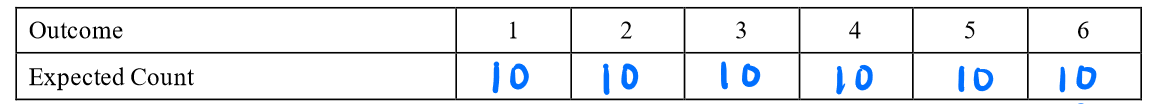
\includegraphics[width=0.8\textwidth]{8.1.1.PNG}
\end{center}

We found the expected count by taking the total number of trials and dividing it equally among each of the outcomes.
\begin{itemize}
    \item An example of an unequal expected count might be the folowing:
    \item An unfair, six-sided die is rolled 60 times. The die is loaded so that the number 1 turns up 50\% of the time and the other five outcomes occur 10\% of the time. What would be the expected count of each outcome?
\end{itemize}
\begin{center}
    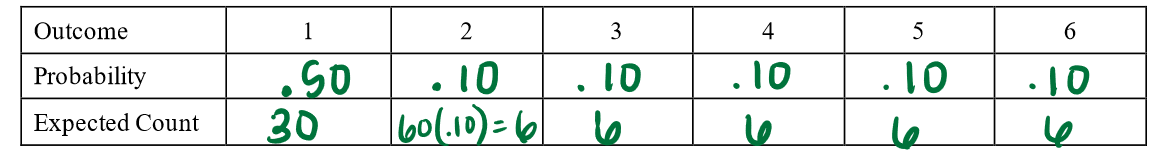
\includegraphics[width=0.8\textwidth]{8.1.2.PNG}
\end{center}

We found the expected count by taking the total number of trials and multiplying it by the probability of the outcome.

Observed Counts:

While we know what is expected, when we run a simulation of rolling a fair die 60 times, we do not expect each outcome to be observed exactly 10 times each due to sampling variability.

Let's say a die was give to you claimed as fair, and you observed the following counts when rolling the die 60 times:
\begin{center}
    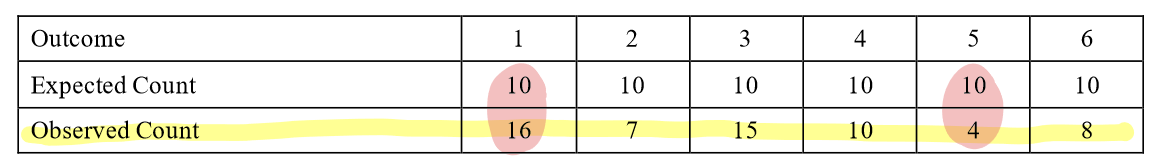
\includegraphics[width=0.8\textwidth]{8.1.3.PNG}
\end{center}
\begin{itemize}
    \item Do you suspect the die given to you was a fair die?
    \item This is going to be the question that our new test helps us answer: Are the differences between the actual observed counts and the expected counts significant?
\end{itemize}

Note: The observed counts must be all whole numbers because they represent actual counts, but the expected counts do not need to be whole numbers.

To measure the difference between the observed and expected counts, and to determine if the difference is significant, we will introduce a new test statistic, called the chi-square statistic:
\[ \chi^2 = \sum \frac{(O-E)^2}{E} \]
Where O represents each observed count in the distribution and E represents each corresponding expected count.
\begin{itemize}
    \item The sampling distribution of the chi-square statistic is not a normal distribution 
    \item It is a right-skewed distribution that allows only for positive values because the statistic cannot be negative.
\end{itemize}

When the expected counts are all at least 5, the sampling distribution of the $\chi^2$ statistic is close to a chi-square distribution with degrees of freedom (df) equal to the number of categories minus 1.
\begin{center}
    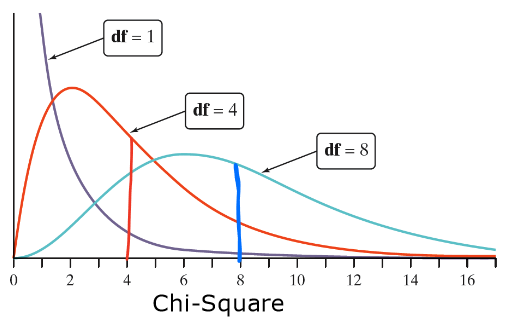
\includegraphics[width=0.8\textwidth]{8.1.4.PNG}
\end{center}
\begin{itemize}
    \item The chi-square distributions are a family of distributions that take only positive values and are skewed to the right.
    \item A particular chi-square distribution is specified by giving its degrees of freedom.
    \item The chi-square goodness-of-fit test uses the chi-square distribution with df = \#categories - 1
\end{itemize}
\begin{center}
    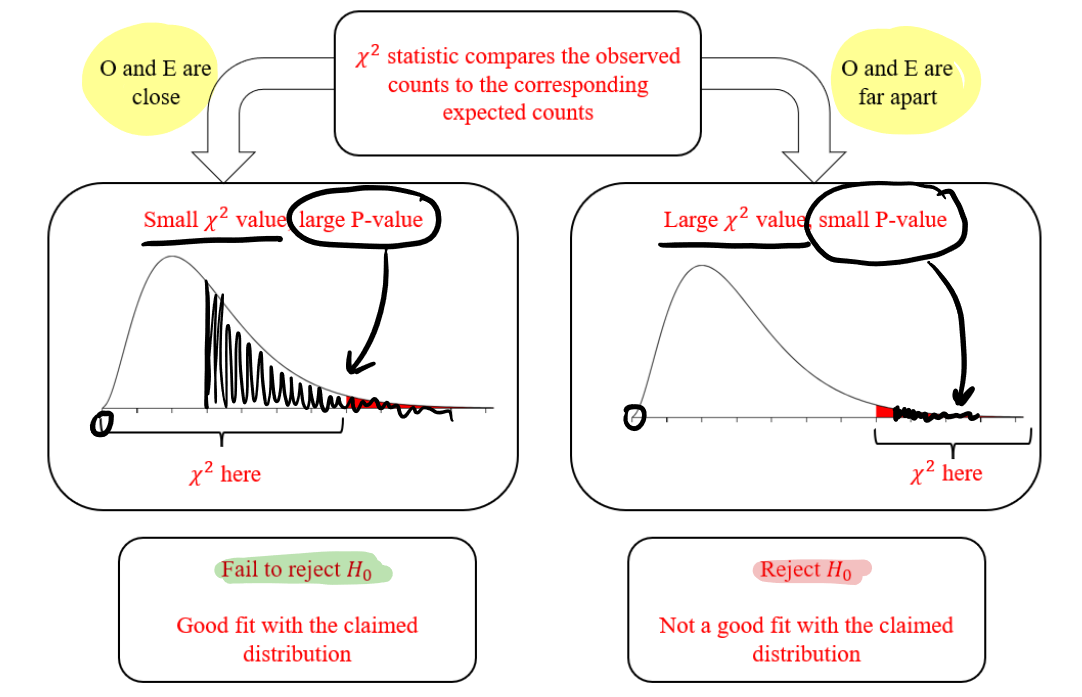
\includegraphics[width=0.8\textwidth]{8.1.5.PNG}
\end{center}

Hypotheses 
\begin{itemize}
    \item The null hypothesis in a chi-square goodness-of-fit test should state a claim about the distribution of a single categorical variable in the population of interest.
    \item We can write this in words or symbols; both are acceptable and used on the AP exam.
    \item Using our fair die as an example, we would say:
\end{itemize}

Using symbols, $H_0: p_1,p_2,p_3,p_4,p_5,p_6 = \frac{1}{6}$, where $p$ is the proportion of outcomes of each face of die.

Using words, $H_0$: The proportion of dice outcomes is equally distributed.

The alternative hypothesis in a chi-square goodness-of-fit test is the categorical variable does not have the specified distribution, and is easily given in words: 

$H_A$: At least one of the claimed proportions is incorrect.

Conditions:
\begin{itemize}
    \item Random: The data came from a well-designed random sample or randomized experiment 
    \item Independent: When sampling without replacement, the 10\% condition is met.
    \item Large Counts
    \begin{itemize}
        \item All expected counts are at least 5
        \item This allows us to say that the sampling distribution will follow a Chi-Square distribution 
    \end{itemize}
\end{itemize}

When the conditions are met, the chi-square goodness of fit test can be performed with the hypotheses:
\begin{center}
    $H_0$: The claimed distribution is correct.
    $H_A$: At least one proportion in the claimed distribution is incorrect.
\end{center}

We find the expected counts assuming the claimed distribution is true, and then we calculate the chi-square statistic:
\[ \chi^2 = \sum \frac{(O-E)^2}{E} \]

The p-value is the area to the right of $\chi^2$ under the density curve of the chi-square distribution with k-1 degrees of freedom, where k represents the number of categories.
\begin{center}
    P-value = P($\chi^2>$ value) = $\chi^2$cdf(value, 1e99, df) on the TI-84
\end{center}

Beware
\begin{enumerate}
    \item The chi-square test statistic compares observed and expected counts. Don't try to perform calculations with the observed and expected proportions in each category.
    \item When checking the Large Counts condition, be sure to examine the expected counts, not the observed.
\end{enumerate}

\pagebreak
\begin{example}
    A geneticist is studying the gene pattern of eye color in a group of white mice. He observed a random sample of mice from the lab and found that 110 had red eyes, 57 had brown eyes, 32 had pink eyes, and 13 had blue eyes. His model suggest that this distribution of eye color should occur in a $9:3:3:1$ ratio. Is there evidence that the geneticist's model is not accurate? Use a 5\% level of significance.

    $H_0$: The proportion of white mice eye color occurs in a $9:3:3:1$ ratio.

    $H_A$: At least one of the proportion is incorrect.

    \begin{itemize}
        \item Random: Random sample of 212 white mice 
        \item Independent: $n=212\leq 0.10$(all white mice)
        \item Large Counts:
    \end{itemize}\medbreak
    \[ \begin{tabular}{c|c|c|c|c}
        & Red & Brown & Pink & Blue \\ \hline 
        OBS & 110 & 57 & 32 & 13\\\hline 
        EXP & 119.25 & 39.75 & 39.75 & 13.25
    \end{tabular}\]

    All expected counts $\geq$ 5.

    Chi Square Test for Goodness of Fit 

    $\chi^2 = \frac{(110-119.25)^2}{119.25}+\frac{(57-39.75)^2}{39.75}+\frac{(32-39.75)^2}{39.75}+\frac{(13-13.25)^2}{13.25}=9.7191$.

    Doing $\chi^2$cdf, with (lower: 9.7191, upper: $\infty$, df: 3) gives $0.0211$ for the p value.

    We can also use a calculator:
    \begin{center}
        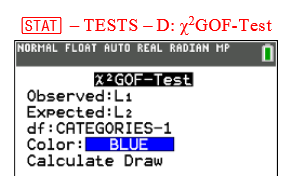
\includegraphics[width=0.4\textwidth]{8.1.6.PNG}
    \end{center}

    Since the p-value of 0.0211 is less than $\alpha=0.05$, we reject the null. There is convincing evidence that the color of white mice eyes does not match a $9:3:3:1$ ratio.
\end{example}


\section{Chi Square Test for Homogeneity}
\begin{itemize}
    \item Recall: The Chi Square Test for Goodness of Fit is testing if one population ``fits'' a given claim.
    \item The Chi Square Test for Homogeneity compares the distributions of one categorical variable across two or more populations to see if they are the same or different 
\end{itemize}

Constructing a Chi-Square Test for Homogeneity:
\begin{itemize}
    \item State the Hypotheses:
    \begin{itemize}
        \item $H_0$: There is no difference in the distribution of {categorical variable} among {two or more groups}.
        \item $H_A$: There is a difference in the distribution of {categorical variable} among {two or more groups}.
    \end{itemize}

    \item Check the Assumptions and Conditions
    \begin{itemize}
        \item Randomness: The individuals whose counts are avaliable for analysis should be a random sample of the population.
        \item 10\% Condition: The sample size, $n$, must be no larger than 10\% of the population.
        \item Large Counts: We should expect to see at least 5 counts in each category of the categorical variable. List the counts and state ``all exp counts $\geq 5$''
    \end{itemize}

    Note: When performing an experiment, Randomness is satisfied by randomly assigning treatments to subjects and the 10\% condition is satisfied if we can assume independence among the individuals in the study.

    \item Name the Inference Method: Chi-Square Test for Homogeneity
    \item Calculate the Test Statistic
    \[ \chi^2 = \sum \frac{\text{(observed-expected)}^2}{\text{expected}} \]
    Observed Counts - Actual frequencies of the variable from your sample 

    Expected Counts - Projected frequencies of the variable if the null hypothesis is true 
    \begin{center}
        EXP = $\frac{\text{row total}\cdot \text{column total}}{\text{table total}}$
    \end{center}

    \item Obtain the P-value 
    2nd-Vars-8:$\chi^2$cdf() 
    \begin{itemize}
        \item Lower: $\chi^2$
        \item Upper: $\infty$
        \item df: (\#Rows-1)(\#Columns-1)
    \end{itemize}

    Calculator Steps:
    \begin{enumerate}
        \item Enter Observed Values into Matrix [A]
        \begin{itemize}
            \item 2nd-$x^{-1}$(Matrix)-EDIT 
            \item \#Rows x \# Columns 
        \end{itemize}
        \item Enter Expected Values into Matrix [B]
        \begin{itemize}
            \item Will populate when you run the $\chi^2$ Test 
        \end{itemize}
        \item STAT-Tests-C:$\chi^2$Test 
        \begin{itemize}
            \item Observed: [A]
            \item Expected: [B]
        \end{itemize}
    \end{enumerate}

    \item Make a decision: This is the same as always 
    \item State your conclusion in context: This is also the same 
\end{itemize}

\pagebreak
\begin{example}
    Andrea is addicted to TikTok and she believes that most students in her high school are too. She wants to investigate if there is a difference in TikTok usage among Juniors and Seniors.
    She randomly samples 65 Juniors and 85 Seniors. The data she collected is given in the table below. Is there convincing evidence of a difference in the distribution of TikTok among the Juniors and Seniors in her school?

    \begin{center}
        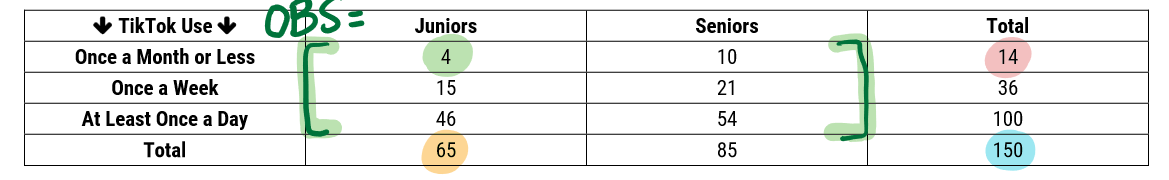
\includegraphics[width=0.8\textwidth]{8.2.1.PNG}
    \end{center}

    $H_0$: TikTok usage among juniors and seniors is the same 

    $H_A$: TikTok usage among juniors and seniors is different.

    \begin{itemize}
        \item Random: Randomly sampled 65 juniors and 85 seniors.
        \item Independent: $65\leq 0.10$(all juniors in her HS), $85\leq 0.10$(all seniors in her HS)
        \item Large Counts: 
        $\begin{bmatrix}
            6.07 & 7.93 \\
            15.6 & 20.4 \\
            43.33 & 56.67
        \end{bmatrix}$
        All exp $\geq 5$

        \item $\chi^2$ Test for Homogeneity
        \item $\chi^2=1.5727$, $p=0.4555$, df = 2: $(\#\text{col}-1)(\#\text{rows}-1)=2$.
        \item Since the p-value of 0.4555 is greater than $\alpha=0.05$, we fail to reject the null. There is not convincing evidence that TikTok usage among juniors and seniors is different at Andrea's high school.
    \end{itemize}
\end{example}
\pagebreak
\begin{example}
    Aspirin prevents blood from clotting which helps prevent strokes. A medical study (we will assume this is a well-designed experiment) asked whether adding another anti-clotting drug named Dipyridamole would be more effective for patients who already had a stroke. Here are the data on strokes during the two years of the study.

    \begin{center}
        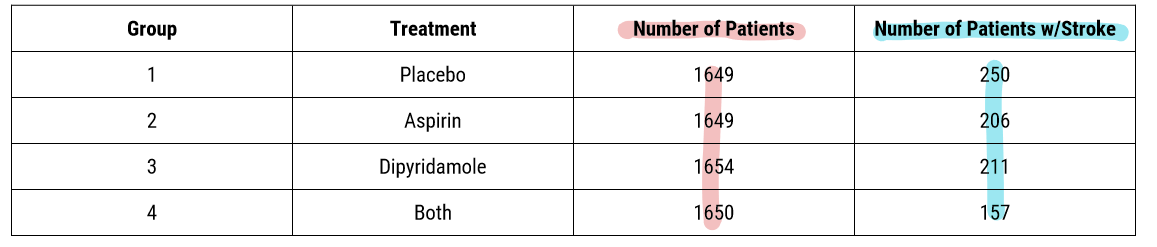
\includegraphics[width=0.8\textwidth]{8.2.2.PNG}
    \end{center}

    (a) Summarize the data into a two-way table.
    \begin{center}
        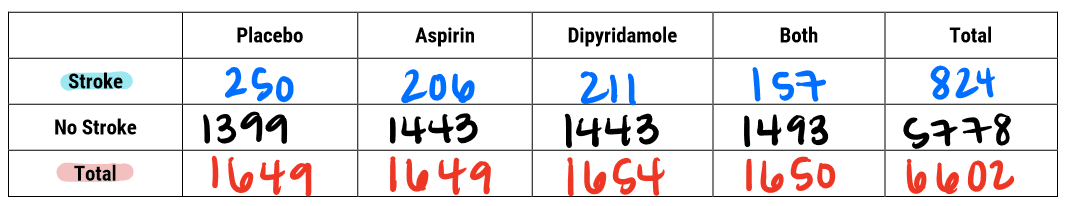
\includegraphics[width=0.8\textwidth]{8.2.3.PNG}
    \end{center}

    (b) Is there convincing evidence of a difference in the effectiveness of the four treatments at the $\alpha=0.05$ significance level?
    \begin{itemize}
        \item $H_0$: No difference in effectiveness among treatments 

        \item $H_A$: Difference in effectiveness among treatments.

        \item Random: Treatments randomly assigned - medical study 
        \item Independent: Assume patient results are independent
        \item Large Counts: EXP = $\begin{bmatrix}
            205.81 & 205.81 & 206.44 & 205.94 \\
            1433.19 & 1433.19 & 1447.56 & 1444.06
        \end{bmatrix}$ All EXP $\geq 5$

        \item $\chi^2$ Test for Homogeneity
        \item $\chi^2 = 24.2428$, $p=0.00002$, df = 3
        \item Since the p-value of 0.00002 is less than $\alpha=0.05$, we reject the null. There is convincing evidence of a difference in effectiveness among the four treatments for preventing strokes.
    \end{itemize}
\end{example}


\section{Chi Square Test for Independence}
\begin{itemize}
    \item Recall: The Chi Square Test for Goodness of Fit is testing is one population ``fits'' a given claim.
    \item Recall: The Chi Square Test for Homogeneity compares the distributions of one categorical variable across two or more populations to see if they are the same or different 
    \item The Chi Square Test for Independence compares the distribution of two categorical variables across one population to see if they are independent (not associated)
\end{itemize}

Constructing a Chi-Square test for Independence:
\begin{itemize}
    \item State the Hypotheses:
    \begin{itemize}
        \item $H_0$: {Categorical Variable 1} and {Categorical Variable 2} are independent (not associated) for {population}
        \item $H_A$: {Categorical Variable 1} and {Categorical Variable 2} are not independent (associated) for {population}
    \end{itemize}
    \item Check Assumptions and Conditions: Same as the test for Homogeneity
    \item Name the Inference Method: Chi-Square Test for Independence
    \item Calculate the Test Statistic: Same as Homogeneity
    \item Obtain the P-Value: This is also the same as Homogeneity
    \item Make Decision: Same as always 
    \item State your conclusion in context: This remains the same 
\end{itemize}

Don't Forget: Association does not imply causation 
\begin{itemize}
    \item A small p-value is not proof of causation.
    \item The Chi Square Test for Independence treats the two variables symmetrically, we cannot differentiate the direction of any possible causation even if it existed.
    \item There is no way to eliminate the possibility that a lurking variable is responsible for the lack of independence.
    \item Don't say that one variable ``depends'' on the other just because they are not independent.
\end{itemize}

\begin{example}
    Andrew thinks there might be a relationship between angry students and GPA. He asks, ``Do students who are prone to sudden bursts of anger have lower GPAs?'' He took an SRS of 300 students at his high school at the beginning of the year. He had each student take the Spielberger Trait Anger Scale Test which measures how 
    prone a person is to sudden anger. At the end of the school year, Andrew collected the data on student GPAs. Here are the results:
    \begin{center}
        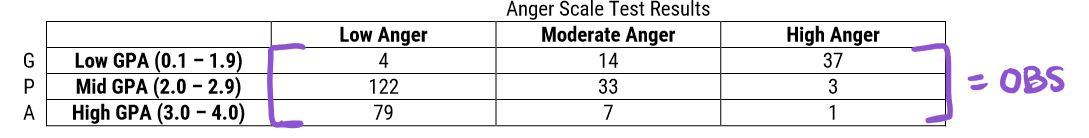
\includegraphics[width=0.8\textwidth]{8.3.1.PNG}
    \end{center}
    Does the data provide convincing evidence of an association between anger level and GPAs at Andrew's HS?

    $H_0$: Anger level and GPA are independent for students at Andrew's HS.

    $H_A$: Anger level and GPA are not independent for students at Andrew's HS.

    \begin{itemize}
        \item Random: SRS Of 300 students at Andrew's HS 
        \item Independent: $n=300\leq 0.10$(all students at Andrew's HS)
        \item Large Counts: $\begin{bmatrix}
            37.58 & 9.90 & 7.52\\
            107.97 & 28.44 & 21.59\\
            59.45&15.66&11.89
        \end{bmatrix}$ All exp counts $\geq 5$
    \end{itemize}
    Chi Square Test for Independence

    $\chi^2=187.1097$, $p\approx 0$ df = 4

    Since the p-value is approx. 0 is less than $\alpha = 0.05$, we reject the null. There is convincing evidence that anger level and GPA are not independent for students at Andrew's HS.
\end{example}

\pagebreak
\begin{example}
    Is your index finger longer than your ring finger? Or is it the other way around? It isn't the same for everyone! To investigate if there is a relationship between gender and relative finger length, we selected a random sample of 460 U.S. high school students who completed a survey. The results are shown in the table below:
    
    \begin{center}
        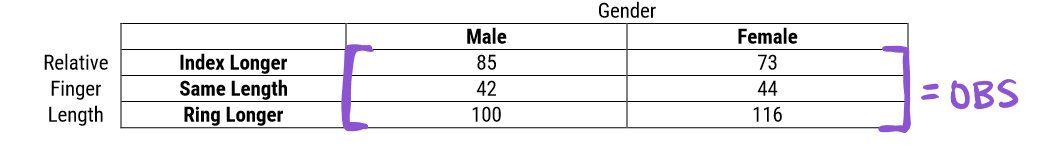
\includegraphics[width=0.8\textwidth]{8.3.2.PNG}
    \end{center}

    $H_0$: Gender and finger length are not associated for US HS Students 

    $H_A$: Gender and finger length are associated for US HS Students 

    \begin{itemize}
        \item Random Sample of 460 US HS Students 
        \item Independent: $n=460\leq 0.10$(all US HS Students)
        \item Large Counts: EXP = $\begin{bmatrix}
            77.97 & 80.03 \\
            42.44 & 43.56 \\
            106.59 & 109.41
        \end{bmatrix}$ All exp counts $\geq 5$
        \item Chi Square Test for Independence
        \item $\chi^2=2.0652$, $p=0.3561$, df = 2
        \item Since the p-value of 0.3561 is greater than $\alpha = 0.05$, we fail to reject the null. There is not convincing evidence that gender and finger length are associated for US HS students.
    \end{itemize}
\end{example}
\end{document}